% Context derivation and target accretion (SPEC.md §8.2).
% Snapshot of the context chain while an `each` element mapping evaluates:
% shared roots are referenced by every level; source/target/paths rebind.
\documentclass[border=8pt]{standalone}
\usepackage[T1]{fontenc}
\usepackage{tikz}
\usetikzlibrary{positioning,arrows.meta,fit}
\begin{document}
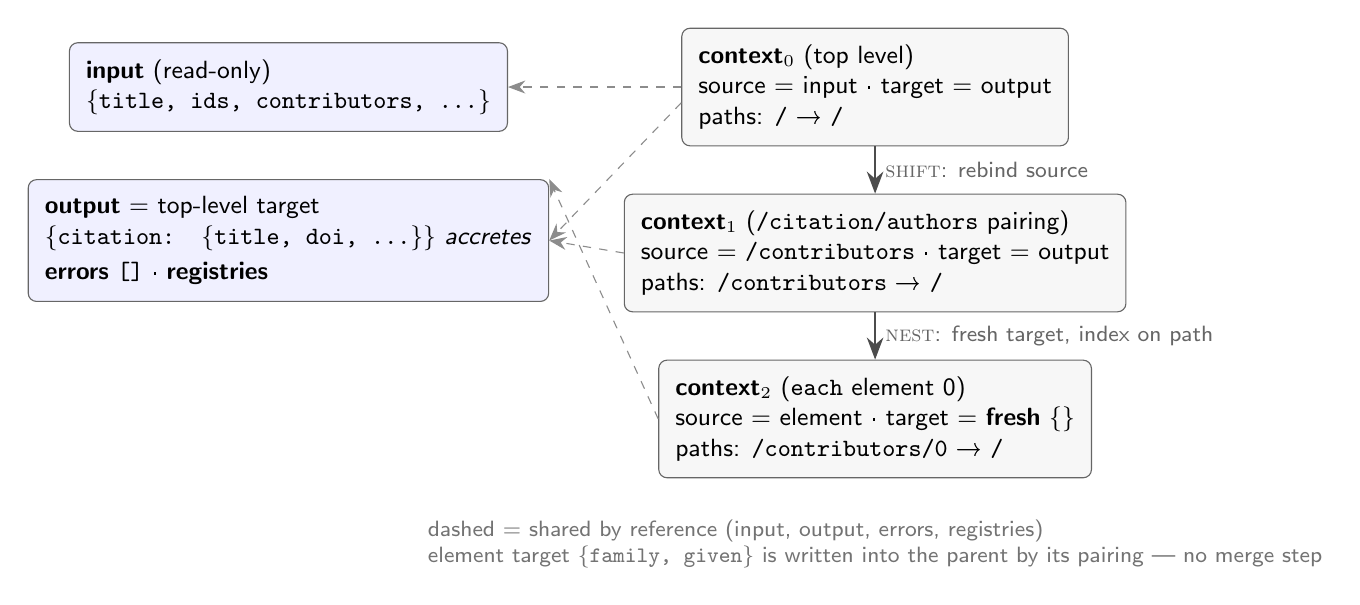
\begin{tikzpicture}[
  font=\sffamily\small,
  ctx/.style={draw=black!60, rounded corners=3pt, align=left, inner sep=6pt, fill=black!3},
  shared/.style={draw=black!60, rounded corners=3pt, align=left, inner sep=6pt, fill=blue!6},
  lbl/.style={font=\sffamily\bfseries\small},
  ref/.style={-{Stealth[length=2.2mm]}, black!45, dashed},
  derive/.style={-{Stealth[length=2.8mm]}, thick, black!70}
]
  % shared roots
  \node[shared] (input) {\textbf{input} (read-only)\\\texttt{\{title, ids, contributors, …\}}};
  \node[shared, below=6mm of input] (output) {\textbf{output} = top-level target\\\texttt{\{citation: \{title, doi, …\}\}} \emph{accretes}\\[2pt]\textbf{errors} \texttt{[]} · \textbf{registries}};

  % context chain
  \node[ctx, right=22mm of input] (c0) {\textbf{context$_0$} (top level)\\source = input · target = output\\paths: \texttt{/} → \texttt{/}};
  \node[ctx, below=6mm of c0] (c1) {\textbf{context$_1$} (\texttt{/citation/authors} pairing)\\source = \texttt{/contributors} · target = output\\paths: \texttt{/contributors} → \texttt{/}};
  \node[ctx, below=6mm of c1] (c2) {\textbf{context$_2$} (\texttt{each} element 0)\\source = element · target = \textbf{fresh} \texttt{\{\}}\\paths: \texttt{/contributors/0} → \texttt{/}};

  \draw[derive] (c0) -- node[right, font=\sffamily\footnotesize, text=black!60] {\textsc{shift}: rebind source} (c1);
  \draw[derive] (c1) -- node[right, font=\sffamily\footnotesize, text=black!60] {\textsc{nest}: fresh target, index on path} (c2);

  \draw[ref] (c0.west) -- (input.east);
  \draw[ref] (c0.west) ++(0,-2mm) -- (output.east);
  \draw[ref] (c1.west) -- (output.east);
  \draw[ref] (c2.west) -- (output.north east);

  \node[font=\sffamily\footnotesize, text=black!55, below=4mm of c2, align=left]
    {dashed = shared by reference (input, output, errors, registries)\\
     element target \texttt{\{family, given\}} is written into the parent by its pairing — no merge step};
\end{tikzpicture}
\end{document}
